\section{Введение}
\subsection{Цель работы}
Цель работы — исследовать зависимость коллекторного тока от напряжения базы в полупроводниковом приборе, вычислить ток насыщения \( I_0 \), а также построить теоретическую кривую зависимости \( I_k = I_0 e^{\frac{e}{kT} U_{\text{эб}}} \) и сравнить её с экспериментальными данными.

\subsection{Решаемые задачи}
\begin{enumerate}
\itemИзмерить зависимость тока короткого замыкания коллектора биполярного
транзистора от напряжения между эмиттером и базой.
\itemПо результатам измерений определить отношение заряда электрона к
постоянной Больцмана.
\end{enumerate}

\section{Основная часть}

\subsection{Теоретическая часть}
Ток короткого замыкания в биполярном транзисторе. Пусть \( U_{\text{ЭБ}} \) — напряжение между эмиттером и базой, \( I_0 \) — ток насыщения, \( T \) — температура в кельвинах, \( e \) — заряд электрона, \( k \) — постоянная Больцмана. Тогда ток короткого замыкания \( I_k \) вычисляется по формуле:

\[
I_k = I_0 \left( e^{\frac{U_{\text{ЭБ}} e}{kT}} - 1 \right)
\]

При комнатной температуре единицей можно пренебречь по сравнению с экспонентой, то есть можно считать:

\[
I_k = I_0 e^{\frac{U_{\text{ЭБ}} e}{kT}}
\]

Прологарифмировав, получим:

\[
\ln I_k = \ln I_0 + \frac{U_{\text{ЭБ}} e}{kT}
\]

График \( \ln I_k \) как функции от \( U_{\text{ЭБ}} \) — прямая. Тангенс угла её наклона равен:

\[
\tan \alpha = \frac{e}{kT}
\]

Откуда:

\[
T = \frac{e}{k \tan \alpha}
\]

Измерения проводились дважды с разными шкалами вольтметра.


\subsection{Эксперимент}
На этой схеме:
\begin{itemize}
    \item БП — блок питания электрической схемы;
    \item \( R_1 \) — ограничительный резистор;
    \item \( R_2 \) — потенциометр, с помощью которого можно изменять напряжение \( U_{\text{эб}} \);
    \item \( V_1 \) — вольтметр для измерения \( U_{\text{эб}} \);
    \item \( R_3 \) — резистор в цепи \( к-б \), по падению напряжения на котором можно измерить ток коллектора \( I_{\text{к}} \);
    \item \( V_2 \) — вольтметр для измерения падения напряжения \( U_{\text{кб}} \) на \( R_3 \).
\end{itemize}.

\begin{figure}[ht!]
\centering
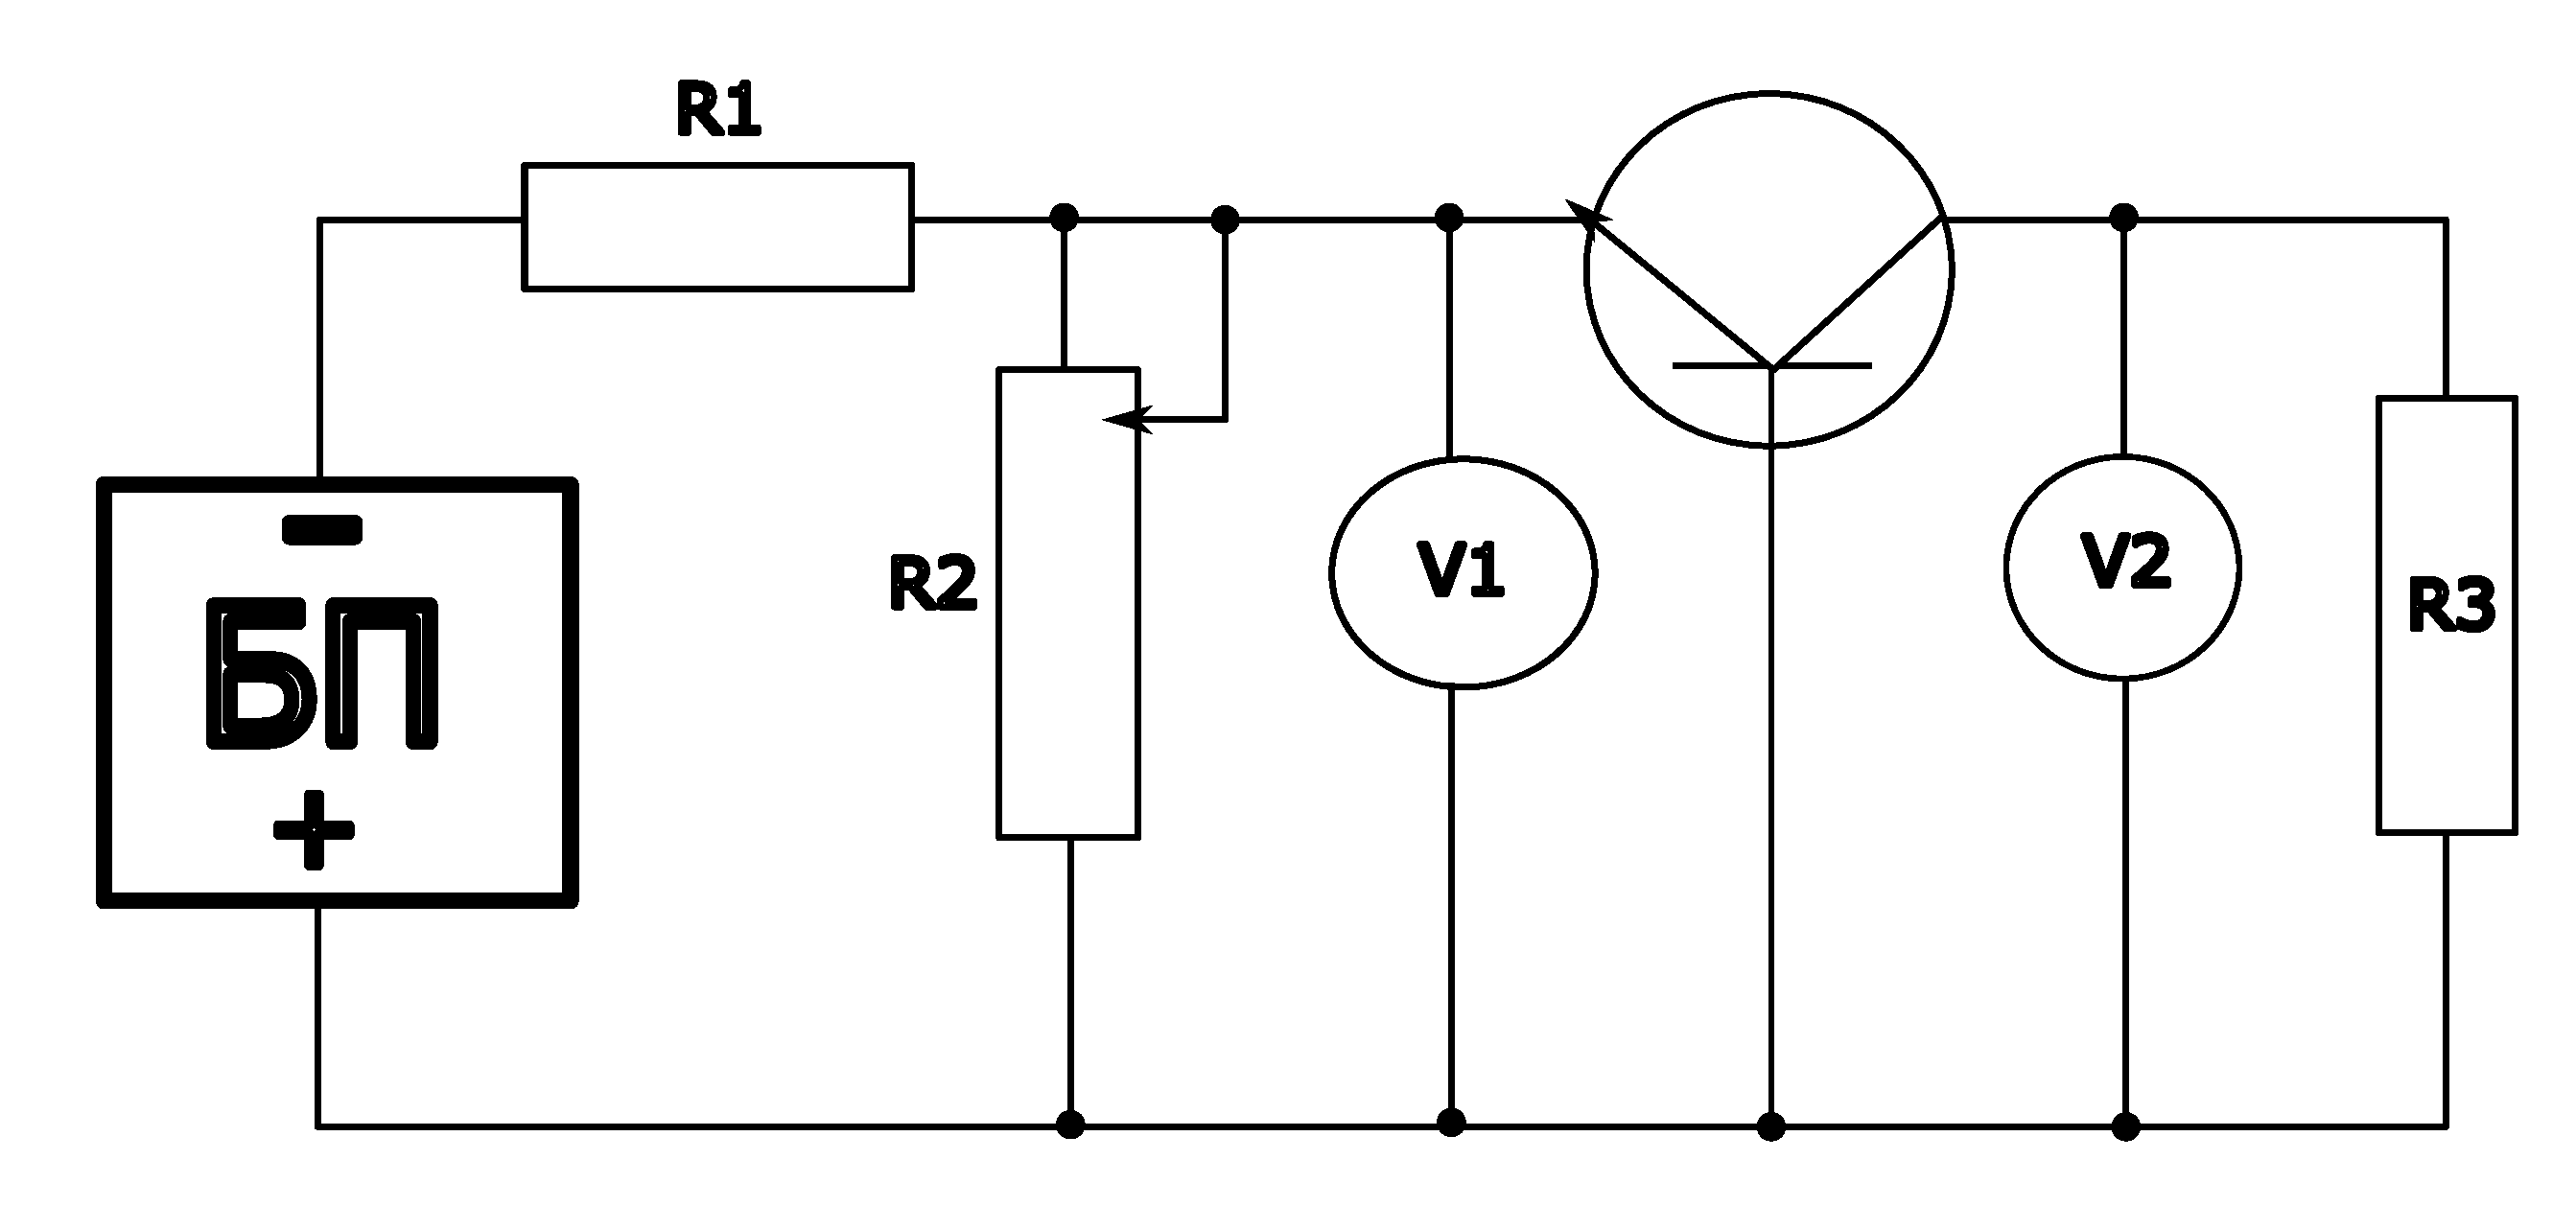
\includegraphics[width=0.9\textwidth]{Схема электрической.pdf}
\caption{Схема электрической установки}
\label{fig:sketch}
\end{figure}

\begin{figure}[H]
\centering
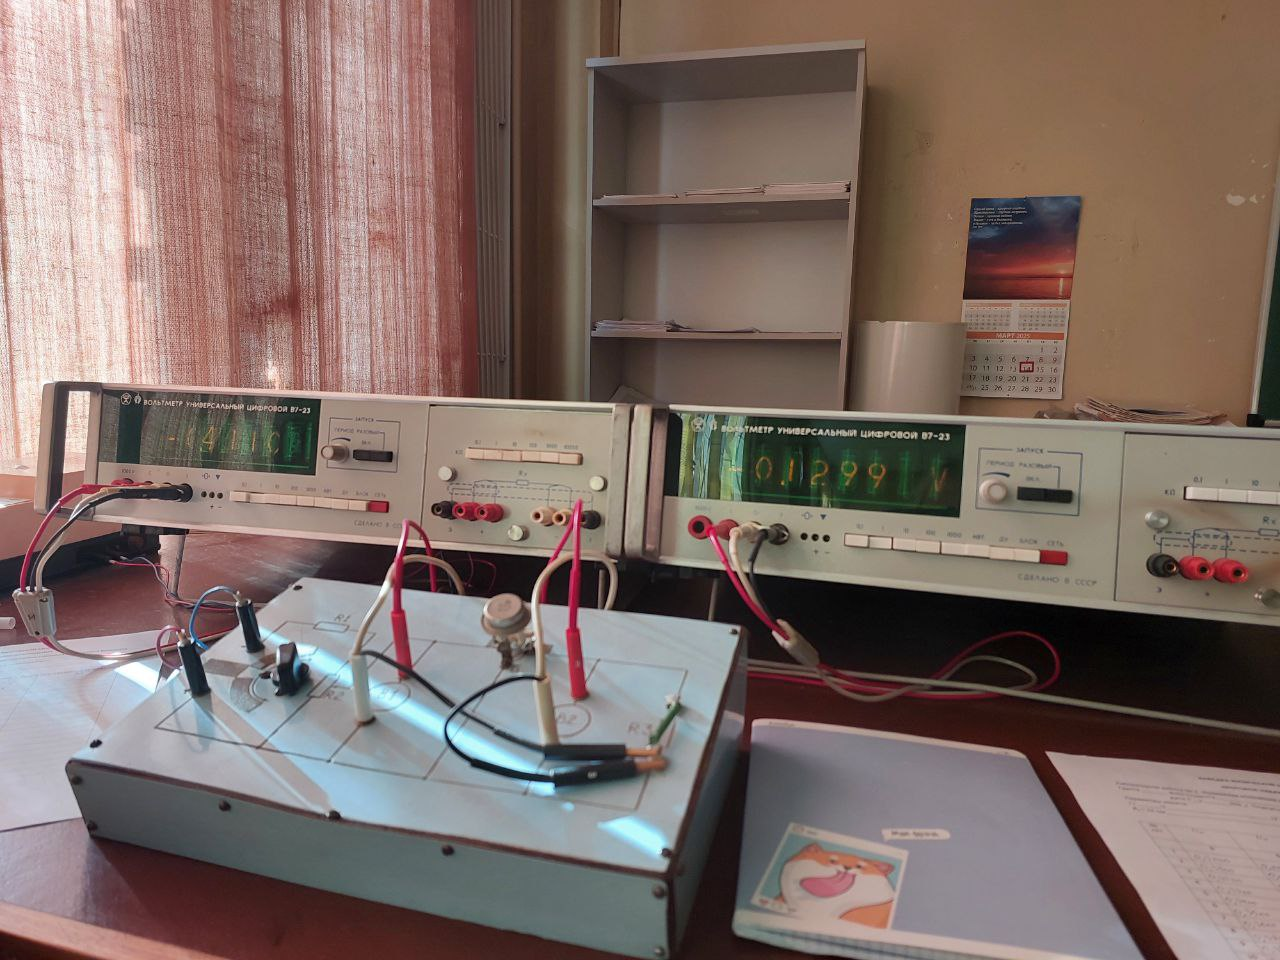
\includegraphics[width=0.6\textwidth]{Установка.jpg}
\caption{Фотография установки}
\label{fig:device}
\end{figure}


\subsection{Обработка данных и обсуждение результатов}

\subsubsection{Исходный код}
Для написания программы, вычисляющей все требуемые данные, используется язык C++; среда разработки - Visual Studio.

Этот код открывает два файла для чтения, один с грубыми данными о напряжениях, а другой с точными. Он извлекает 16 значений напряжений из каждого файла и сохраняет их в два вектора: Urough для грубых данных и Uprecise для точных. Затем программа вычисляет токи, где напряжение делится на 12, а результат умножается на 1000 для перевода в миллиамперы.
После этого программа вычисляет натуральный логарифм тока и записывает результаты в четыре файла: два для значений тока (для грубых и точных данных) и два для значений их логарифмов. В конце работы программы все файлы закрываются, и выводится сообщение, что результаты успешно сохранены в соответствующие файлы.

\begin{lstlisting}[label=listing1, caption=Функция вычисления тока]
 // Массивы для хранения значений Iк для грубых и точных измерений
    std::vector<double> Irough(16);
    std::vector<double> Iprecise(16);

    // Вычисляем Iк для грубых и точных измерений и переводим в мА
    for (int i = 0; i < 16; ++i) {
        Irough[i] = (Urough[i] / 12.0) * 1000;   // Iк = Uк / 12 и переводим в мА (грубые данные)
        Iprecise[i] = (Uprecise[i] / 12.0) * 1000; // Iк = Uк / 12 и переводим в мА (точные данные)
\end{lstlisting}

Этот код выполняет анализ данных с использованием метода парных точек. Он считывает данные из двух файлов, вычисляет наклон для каждой пары точек, а затем проводит статистический анализ этих наклонов. Для каждой пары точек рассчитываются разницы по координатам \( x \) и \( y \), а затем вычисляется наклон \( a_i = \frac{dy}{dx} \). Результаты выводятся в консоль и записываются в файл CSV.

\[
a_i = \frac{dy}{dx}
\]

Далее программа вычисляет среднее значение наклона \( \bar{a} \), отклонения от среднего для каждого значения \( a_i - \bar{a} \), а также квадраты отклонений \( (a_i - \bar{a})^2 \). Эти величины используются для вычисления стандартного отклонения и стандартной ошибки, а также 95\% доверительного интервала для наклона \( [a_{\text{min}}, a_{\text{max}}] \).

\[
\bar{a} = \frac{1}{N} \sum_{i=1}^{N} a_i
\]

\[
\sigma = \sqrt{\frac{1}{N-1} \sum_{i=1}^{N} (a_i - \bar{a})^2}
\]
Для расчетов используется t-критическое значение для 95\% доверия:

\[
t_{\text{value}} = 2.3646
\]

\begin{lstlisting}[label=listing2, caption=Функция расчета отклонений]
    for (int i = 0; i < N; ++i) {
        double diff = a[i] - a_avg;
        double diff_sq = diff * diff;
        sum_diff += diff;
        sum_diff_sq += diff_sq;

        cout << i + 1 << ";" << a[i] << ";" << diff << ";" << diff_sq << endl;
        outfile << i + 1 << ";" << a[i] << ";" << diff << ";" << diff_sq << "\n";
    }

    double variance = sum_diff_sq / (N - 1);
    double std_dev = sqrt(variance);
    double std_err = std_dev / sqrt(N);
    double delta_a = t_value * std_err;

    double a_min = a_avg - delta_a;
    double a_max = a_avg + delta_a;

    double ek = T * a_avg;
    double delta_ek = T * delta_a;
\end{lstlisting}

Аналогично и для точных измерений

\subsubsection{Таблицы}

\begin{longtable}{|c|c|c|c|c|}
\hline
№п/п & $U_{\text{эб}}$, В & $U_{\text{кб}}$, В & $I_k = \frac{U_{\text{кб}}}{R_3}$, мА & $\ln I_k$ \\
\hline
\endfirsthead
\hline
№п/п & $U_{эб}$, В & $U_{кб}$, В & $I_k = \frac{U_{кб}}{R_3}$, мА & $\ln I_k$ \\
\hline
\endhead
\hline
1 & 0.30 & 0.0019 & 0.158333 & -8.750810 \\
2 & 0.31 & 0.0038 & 0.316667 & -8.057660 \\
3 & 0.32 & 0.0073 & 0.608333 & -7.404790 \\
4 & 0.33 & 0.0106 & 0.883333 & -7.031810 \\
5 & 0.34 & 0.0165 & 1.375000 & -6.589300 \\
6 & 0.35 & 0.0257 & 2.141670 & -6.146170 \\
7 & 0.36 & 0.0424 & 3.533330 & -5.645510 \\
8 & 0.37 & 0.0550 & 4.583330 & -5.385330 \\
9 & 0.38 & 0.0761 & 6.341670 & -5.060610 \\
10 & 0.39 & 0.0910 & 7.583330 & -4.881800 \\
11 & 0.40 & 0.1215 & 10.125000 & -4.592750 \\
12 & 0.41 & 0.1502 & 12.516700 & -4.380690 \\
13 & 0.42 & 0.1864 & 15.533300 & -4.164770 \\
14 & 0.43 & 0.2126 & 17.716700 & -4.033250 \\
15 & 0.44 & 0.2308 & 19.233300 & -3.951110 \\
16 & 0.45 & 0.2530 & 21.083300 & -3.859270 \\
\hline
\caption{Грубые измерения}
\end{longtable}

\begin{longtable}{|c|c|c|c|c|c|c|c|c|c|}
\hline
№ & $x_2$ & $x_1$ & $x_2 - x_1$ & $y_2$ & $y_1$ & $y_2 - y_1$ & $a_i$ & $a_i - a$ & $(a_i - a)^2$ \\
\hline
\endhead
\hline
1 & 0.380 & 0.300 & 0.080 & -5.061 & -8.751 & 3.690 & 46.128 & 14.741 & 217.308 \\
2 & 0.390 & 0.310 & 0.080 & -4.882 & -8.058 & 3.176 & 39.698 & 8.312 & 69.091 \\
3 & 0.400 & 0.320 & 0.080 & -4.593 & -7.405 & 2.812 & 35.151 & 3.764 & 14.170 \\
4 & 0.410 & 0.330 & 0.080 & -4.381 & -7.032 & 2.651 & 33.139 & 1.753 & 3.073 \\
5 & 0.420 & 0.340 & 0.080 & -4.165 & -6.589 & 2.425 & 30.307 & -1.080 & 1.165 \\
6 & 0.430 & 0.350 & 0.080 & -4.033 & -6.146 & 2.113 & 26.412 & -4.975 & 24.747 \\
7 & 0.440 & 0.360 & 0.080 & -3.951 & -5.646 & 1.694 & 21.180 & -10.206 & 104.165 \\
8 & 0.450 & 0.370 & 0.080 & -3.859 & -5.385 & 1.526 & 19.076 & -12.310 & 151.546 \\
\hline
\caption{Метод парных точек для грубых измерений}
\end{longtable}

Среднее значение a=31.386
Рассчитаем стандартную погрешность выборки по формуле:
\[
S = \sqrt{\frac{\sum (a_i - \bar{a})^2}{n(n-1)}}
\]
где \(S\) — стандартная погрешность выборки, \(a_i\) — значения наблюдений, \(\bar{a}\) — среднее значение, \(n\) — количество элементов в выборке.

S=3.233 1/В


Найдем коэффициент Стьюдента t для 8 элементов и вероятности 0,95 из таблиц: t = 2,3646
\[
\tan(\alpha) = 31,386 \pm 7,644 \, \left(\frac{1}{\text{В}}\right)
\]

Определим теперь погрешность измерения искомого отношения как погрешность косвенных измерений по формуле
\[
\Delta \frac{e}{k} = \sqrt{\frac{1}{9} \left( \frac{\partial \frac{e}{k}}{\partial T} \right)^2 \Delta T^2 + \left( \frac{\partial \frac{e}{k}}{\partial \tan \alpha} \right)^2 \Delta \tan \alpha^2 }
\]

\[
\Delta \frac{e}{k} = \sqrt{\frac{1}{9} \bar{a}^2 \Delta T^2 + T^2 \Delta \tan \alpha^2} \tag{4}
\]

Где:
\[
\Delta T = 0.5 \, \text{K}, \quad \Delta \tan \alpha = S \cdot t = 7,645 \, \frac{1}{\text{В}}
\]

Тогда для первого измерения:
\[
\frac{e}{k} = (9321.684 \pm 870.369)~\frac{\text{К}}{\text{В}}
\]

Далее рассчитаем ток насыщения по формуле:
\[
I_0 = \exp\left( \overline{\ln I_k} - \frac{e}{kT} \cdot \overline{U_{\text{эб}}} \right)
\]


Таким образом, значение тока насыщения равно:
\[
I_0 = 2.801 \times 10^{-8}~\text{мА}
\]





\begin{longtable}{|c|c|c|c|c|}
\hline
№п/п & $U_{\text{эб}}$, В & $U_{\text{кб}}$, В & $I_k = \frac{U_{\text{кб}}}{R_3}$, мА & $\ln I_k$ \\
\hline
\endfirsthead
\hline
№п/п & $U_{эб}$, В & $U_{кб}$, В & $I_k = \frac{U_{кб}}{R_3}$, мА & $\ln I_k$ \\
\hline
\endhead
\hline
1 & 0.3000 & 0.0017 & 0.141667 & -8.862030 \\
2 & 0.3100 & 0.0029 & 0.241667 & -8.327950 \\
3 & 0.3200 & 0.0055 & 0.458333 & -7.687910 \\
4 & 0.3300 & 0.0104 & 0.866667 & -7.050860 \\
5 & 0.3400 & 0.0142 & 1.183330 & -6.739420 \\
6 & 0.3500 & 0.0241 & 2.008330 & -6.210450 \\
7 & 0.3600 & 0.0360 & 3.000000 & -5.809140 \\
8 & 0.3700 & 0.0485 & 4.041670 & -5.511100 \\
9 & 0.3800 & 0.0666 & 5.550000 & -5.193960 \\
10 & 0.3900 & 0.0888 & 7.400000 & -4.906280 \\
11 & 0.4000 & 0.1114 & 9.283330 & -4.679530 \\
12 & 0.4100 & 0.1414 & 11.783300 & -4.441070 \\
13 & 0.4200 & 0.1709 & 14.241700 & -4.251580 \\
14 & 0.4300 & 0.1979 & 16.491700 & -4.104900 \\
15 & 0.4400 & 0.22256 & 18.800000 & -3.973900 \\
16 & 0.4500 & 0.2470 & 20.583300 & -3.883270 \\
\hline
\caption{Точные измерения}
\end{longtable}



\begin{longtable}{|c|c|c|c|c|c|c|c|c|c|}
\hline
№ & $x_2$ & $x_1$ & $x_2 - x_1$ & $y_2$ & $y_1$ & $y_2 - y_1$ & $a_i$ & $a_i - a$ & $(a_i - a)^2$ \\
\hline
\endhead
\hline
1 & 0.380 & 0.300 & 0.080 & -5.194 & -8.862 & 3.668 & 45.851 & 13.407 & 179.735 \\
2 & 0.390 & 0.310 & 0.080 & -4.906 & -8.328 & 3.422 & 42.771 & 10.327 & 106.638 \\
3 & 0.400 & 0.320 & 0.080 & -4.680 & -7.688 & 3.008 & 37.605 & 5.160 & 26.630 \\
4 & 0.410 & 0.330 & 0.080 & -4.441 & -7.051 & 2.610 & 32.622 & 0.178 & 0.032 \\
5 & 0.420 & 0.340 & 0.080 & -4.252 & -6.739 & 2.488 & 31.098 & -1.346 & 1.813 \\
6 & 0.430 & 0.350 & 0.080 & -4.105 & -6.210 & 2.106 & 26.319 & -6.125 & 37.515 \\
7 & 0.440 & 0.360 & 0.080 & -3.974 & -5.809 & 1.835 & 22.941 & -9.504 & 90.323 \\
8 & 0.450 & 0.370 & 0.080 & -3.883 & -5.511 & 1.628 & 20.348 & -12.096 & 146.324 \\
\hline
\caption{Метод парных точек для точных измерений}
\end{longtable}

Аналогично S=3.243 1/В

Среднее a=32.444

\[
\tan(\alpha) = 32,443 \pm 7,669 \, \left(\frac{1}{\text{В}}\right)
\]
\[
\frac{e}{k} = (9635.965 \pm 877.620)~\frac{\text{К}}{\text{В}}
\]

Ток насыщения:
\[
I_0 = 1.694 \times 10^{-8}~\text{мА}
\]


\subsubsection{Графики}


\begin{figure}[H]
\centering
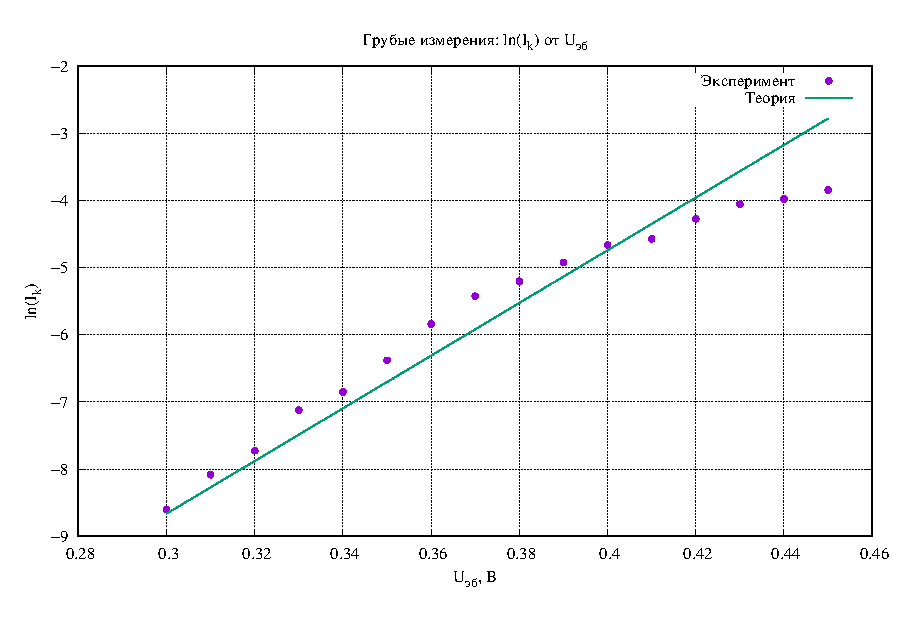
\includegraphics[width=0.6\textwidth]{plot1_3.eps}
\caption{График}
\label{fig:device}
\end{figure}


\begin{figure}[H]
\centering
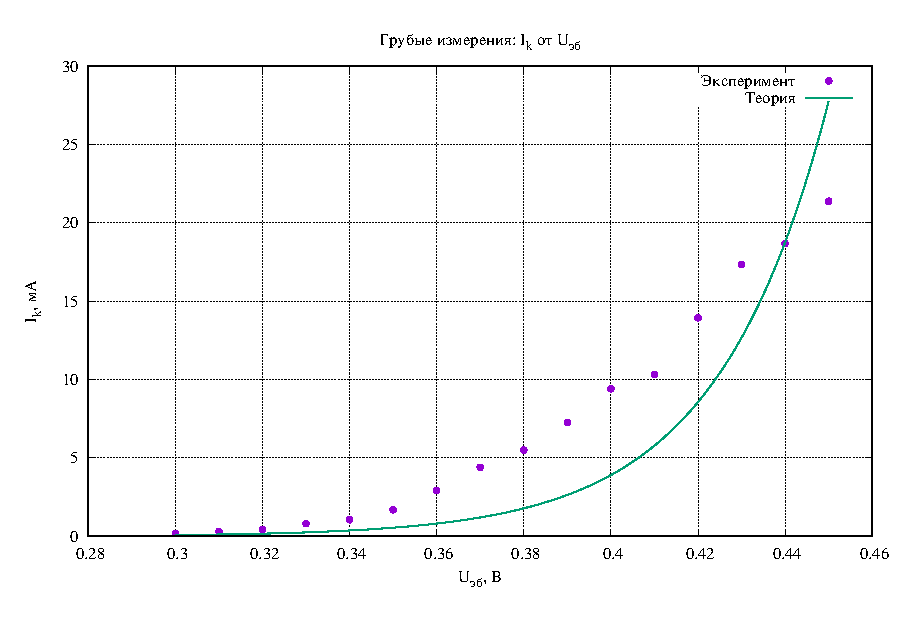
\includegraphics[width=0.6\textwidth]{plot2_3.eps}
\caption{График}
\label{fig:device}
\end{figure}


\begin{figure}[H]
\centering
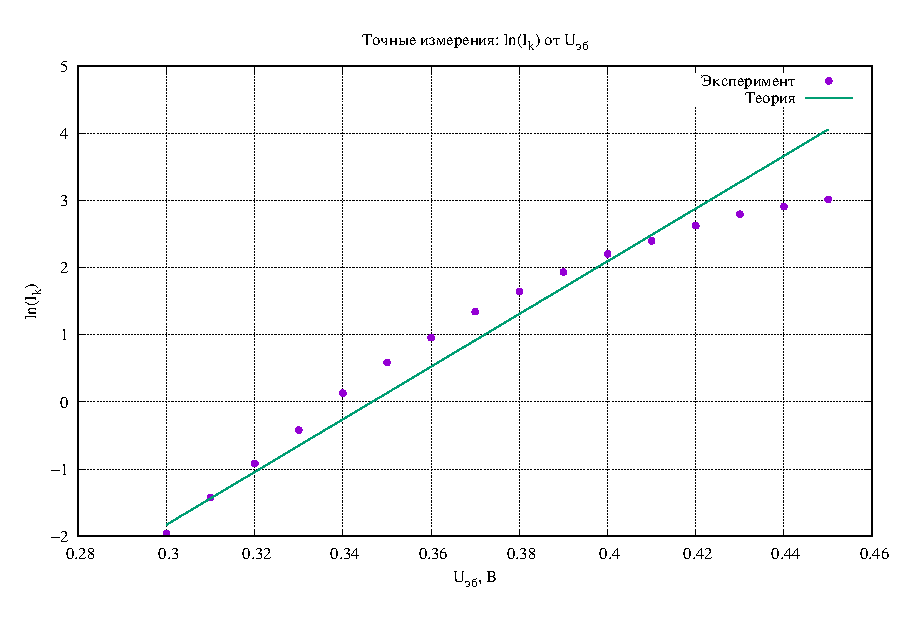
\includegraphics[width=0.6\textwidth]{plot3_3.eps}
\caption{График}
\label{fig:device}
\end{figure}


\begin{figure}[H]
\centering
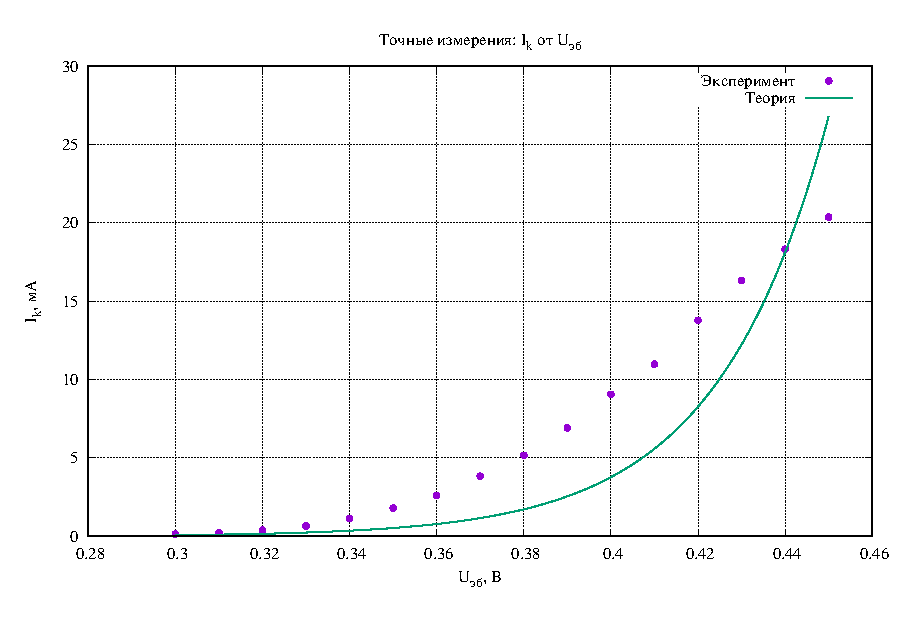
\includegraphics[width=0.6\textwidth]{plot4_3.eps}
\caption{График}
\label{fig:device}
\end{figure}


\section{Вывод}
В ходе экспериментальных исследований было проведено измерение отношения заряда электрона к постоянной Больцмана. Кроме того, изучена зависимость тока короткого замыкания коллектора биполярного транзистора от напряжения между эмиттером и базой, по результатам измерений построены соответствующие графические зависимости.

Погрешность определения искомой физической постоянной рассчитана методом оценки погрешностей косвенных измерений. Полученные результаты находятся в удовлетворительном согласии с теоретическими предсказаниями, что подтверждает корректность применённой методики измерений.

Данные исследования позволяют сделать вывод о применимости использованного экспериментального подхода для определения фундаментальных физических констант и изучения характеристик полупроводниковых приборов.

% Список литературы
% Для отчёта он не обязателен
\begin{thebibliography}{9}

%ссылка на репозиторий с исходныим кодом отчета и всех расчетных программ обязательна 
\bibitem{repo}
\url{https://github.com/st117168/2025-4sem-Measurement_methods/tree/main/Workshop4} 

\end{thebibliography}

\appendix